% topic3.tex -- Module 7 Topic 3: Light: quantum model, Q37-54.
\topictitle{Topic 3 - Light: Quantum Model}

% ---- Q37 (black-body curves)
\begin{quizq}{}
Which graph correctly shows the black-body radiation curves for a hotter object (solid line) and a
cooler object (dashed line)?
\gridopts{%
  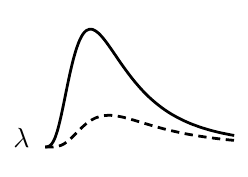
\begin{tikzpicture}\gaxesP{Intensity}{$\lambda$}
    \draw[line width=1pt, smooth] plot coordinates {(0.20,0.001) (0.24,0.008) (0.28,0.037) (0.32,0.107) (0.36,0.225) (0.40,0.388) (0.44,0.577) (0.48,0.774) (0.52,0.961) (0.56,1.125) (0.60,1.260) (0.64,1.364) (0.68,1.436) (0.72,1.479) (0.76,1.497) (0.80,1.495) (0.84,1.476) (0.88,1.444) (0.92,1.402) (0.96,1.353) (1.00,1.299) (1.04,1.242) (1.08,1.184) (1.12,1.125) (1.16,1.067) (1.20,1.011) (1.24,0.956) (1.28,0.903) (1.32,0.852) (1.36,0.804) (1.40,0.758) (1.44,0.714) (1.48,0.673) (1.52,0.634) (1.56,0.598) (1.60,0.564) (1.64,0.532) (1.68,0.501) (1.72,0.473) (1.76,0.446) (1.80,0.421) (1.84,0.398) (1.88,0.376) (1.92,0.356) (1.96,0.336) (2.00,0.318) (2.04,0.301) (2.08,0.285) (2.12,0.271) (2.16,0.256) (2.20,0.243) (2.24,0.231) (2.28,0.219) (2.32,0.208) (2.36,0.198) (2.40,0.188) (2.44,0.179) (2.48,0.171) (2.52,0.163) (2.56,0.155) (2.60,0.148)};
    \draw[line width=1pt, dash pattern=on 3pt off 2pt, smooth] plot coordinates {(0.20,0.000) (0.24,0.000) (0.28,0.001) (0.32,0.003) (0.36,0.009) (0.40,0.022) (0.44,0.042) (0.48,0.070) (0.52,0.104) (0.56,0.143) (0.60,0.184) (0.64,0.224) (0.68,0.262) (0.72,0.297) (0.76,0.326) (0.80,0.351) (0.84,0.371) (0.88,0.385) (0.92,0.396) (0.96,0.401) (1.00,0.404) (1.04,0.403) (1.08,0.399) (1.12,0.393) (1.16,0.386) (1.20,0.377) (1.24,0.366) (1.28,0.355) (1.32,0.344) (1.36,0.332) (1.40,0.320) (1.44,0.308) (1.48,0.296) (1.52,0.284) (1.56,0.272) (1.60,0.261) (1.64,0.250) (1.68,0.239) (1.72,0.228) (1.76,0.218) (1.80,0.209) (1.84,0.200) (1.88,0.191) (1.92,0.182) (1.96,0.174) (2.00,0.166) (2.04,0.159) (2.08,0.152) (2.12,0.145) (2.16,0.139) (2.20,0.133) (2.24,0.127) (2.28,0.121) (2.32,0.116) (2.36,0.111) (2.40,0.106) (2.44,0.102) (2.48,0.097) (2.52,0.093) (2.56,0.089) (2.60,0.086)};
  \end{tikzpicture}}
  {%
  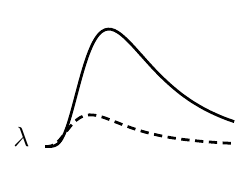
\begin{tikzpicture}\gaxesP{Intensity}{$\lambda$}
    \draw[line width=1pt, smooth] plot coordinates {(0.20,0.000) (0.24,0.000) (0.28,0.002) (0.32,0.011) (0.36,0.034) (0.40,0.080) (0.44,0.155) (0.48,0.258) (0.52,0.386) (0.56,0.530) (0.60,0.680) (0.64,0.829) (0.68,0.970) (0.72,1.097) (0.76,1.207) (0.80,1.299) (0.84,1.371) (0.88,1.425) (0.92,1.462) (0.96,1.484) (1.00,1.492) (1.04,1.489) (1.08,1.476) (1.12,1.454) (1.16,1.426) (1.20,1.392) (1.24,1.355) (1.28,1.314) (1.32,1.272) (1.36,1.228) (1.40,1.183) (1.44,1.139) (1.48,1.094) (1.52,1.050) (1.56,1.006) (1.60,0.964) (1.64,0.923) (1.68,0.883) (1.72,0.845) (1.76,0.808) (1.80,0.772) (1.84,0.738) (1.88,0.705) (1.92,0.673) (1.96,0.643) (2.00,0.615) (2.04,0.587) (2.08,0.561) (2.12,0.537) (2.16,0.513) (2.20,0.490) (2.24,0.469) (2.28,0.448) (2.32,0.429) (2.36,0.411) (2.40,0.393) (2.44,0.376) (2.48,0.360) (2.52,0.345) (2.56,0.331) (2.60,0.317)};
    \draw[line width=1pt, dash pattern=on 3pt off 2pt, smooth] plot coordinates {(0.20,0.000) (0.24,0.002) (0.28,0.010) (0.32,0.029) (0.36,0.061) (0.40,0.104) (0.44,0.155) (0.48,0.208) (0.52,0.258) (0.56,0.303) (0.60,0.339) (0.64,0.367) (0.68,0.386) (0.72,0.398) (0.76,0.403) (0.80,0.402) (0.84,0.397) (0.88,0.388) (0.92,0.377) (0.96,0.364) (1.00,0.349) (1.04,0.334) (1.08,0.318) (1.12,0.303) (1.16,0.287) (1.20,0.272) (1.24,0.257) (1.28,0.243) (1.32,0.229) (1.36,0.216) (1.40,0.204) (1.44,0.192) (1.48,0.181) (1.52,0.171) (1.56,0.161) (1.60,0.152) (1.64,0.143) (1.68,0.135) (1.72,0.127) (1.76,0.120) (1.80,0.113) (1.84,0.107) (1.88,0.101) (1.92,0.096) (1.96,0.090) (2.00,0.086) (2.04,0.081) (2.08,0.077) (2.12,0.073) (2.16,0.069) (2.20,0.065) (2.24,0.062) (2.28,0.059) (2.32,0.056) (2.36,0.053) (2.40,0.051) (2.44,0.048) (2.48,0.046) (2.52,0.044) (2.56,0.042) (2.60,0.040)};
  \end{tikzpicture}}
  {%
  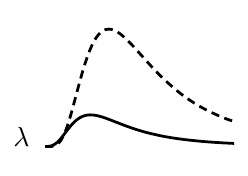
\begin{tikzpicture}\gaxesP{Intensity}{$\lambda$}
    \draw[line width=1pt, smooth] plot coordinates {(0.20,0.000) (0.24,0.002) (0.28,0.010) (0.32,0.029) (0.36,0.061) (0.40,0.104) (0.44,0.155) (0.48,0.208) (0.52,0.258) (0.56,0.303) (0.60,0.339) (0.64,0.367) (0.68,0.386) (0.72,0.398) (0.76,0.403) (0.80,0.402) (0.84,0.397) (0.88,0.388) (0.92,0.377) (0.96,0.364) (1.00,0.349) (1.04,0.334) (1.08,0.318) (1.12,0.303) (1.16,0.287) (1.20,0.272) (1.24,0.257) (1.28,0.243) (1.32,0.229) (1.36,0.216) (1.40,0.204) (1.44,0.192) (1.48,0.181) (1.52,0.171) (1.56,0.161) (1.60,0.152) (1.64,0.143) (1.68,0.135) (1.72,0.127) (1.76,0.120) (1.80,0.113) (1.84,0.107) (1.88,0.101) (1.92,0.096) (1.96,0.090) (2.00,0.086) (2.04,0.081) (2.08,0.077) (2.12,0.073) (2.16,0.069) (2.20,0.065) (2.24,0.062) (2.28,0.059) (2.32,0.056) (2.36,0.053) (2.40,0.051) (2.44,0.048) (2.48,0.046) (2.52,0.044) (2.56,0.042) (2.60,0.040)};
    \draw[line width=1pt, dash pattern=on 3pt off 2pt, smooth] plot coordinates {(0.20,0.000) (0.24,0.000) (0.28,0.002) (0.32,0.011) (0.36,0.034) (0.40,0.080) (0.44,0.155) (0.48,0.258) (0.52,0.386) (0.56,0.530) (0.60,0.680) (0.64,0.829) (0.68,0.970) (0.72,1.097) (0.76,1.207) (0.80,1.299) (0.84,1.371) (0.88,1.425) (0.92,1.462) (0.96,1.484) (1.00,1.492) (1.04,1.489) (1.08,1.476) (1.12,1.454) (1.16,1.426) (1.20,1.392) (1.24,1.355) (1.28,1.314) (1.32,1.272) (1.36,1.228) (1.40,1.183) (1.44,1.139) (1.48,1.094) (1.52,1.050) (1.56,1.006) (1.60,0.964) (1.64,0.923) (1.68,0.883) (1.72,0.845) (1.76,0.808) (1.80,0.772) (1.84,0.738) (1.88,0.705) (1.92,0.673) (1.96,0.643) (2.00,0.615) (2.04,0.587) (2.08,0.561) (2.12,0.537) (2.16,0.513) (2.20,0.490) (2.24,0.469) (2.28,0.448) (2.32,0.429) (2.36,0.411) (2.40,0.393) (2.44,0.376) (2.48,0.360) (2.52,0.345) (2.56,0.331) (2.60,0.317)};
  \end{tikzpicture}}
  {%
  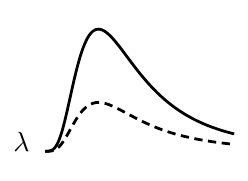
\begin{tikzpicture}\gaxesP{Intensity}{$\lambda$}
    \draw[line width=1pt, smooth] plot coordinates {(0.20,0.000) (0.24,0.002) (0.28,0.012) (0.32,0.043) (0.36,0.107) (0.40,0.211) (0.44,0.353) (0.48,0.520) (0.52,0.700) (0.56,0.878) (0.60,1.044) (0.64,1.190) (0.68,1.311) (0.72,1.406) (0.76,1.476) (0.80,1.522) (0.84,1.546) (0.88,1.553) (0.92,1.544) (0.96,1.523) (1.00,1.491) (1.04,1.452) (1.08,1.408) (1.12,1.359) (1.16,1.308) (1.20,1.255) (1.24,1.201) (1.28,1.147) (1.32,1.095) (1.36,1.043) (1.40,0.992) (1.44,0.944) (1.48,0.897) (1.52,0.852) (1.56,0.809) (1.60,0.768) (1.64,0.728) (1.68,0.691) (1.72,0.656) (1.76,0.622) (1.80,0.591) (1.84,0.561) (1.88,0.532) (1.92,0.506) (1.96,0.480) (2.00,0.456) (2.04,0.434) (2.08,0.412) (2.12,0.392) (2.16,0.373) (2.20,0.355) (2.24,0.338) (2.28,0.322) (2.32,0.307) (2.36,0.293) (2.40,0.279) (2.44,0.266) (2.48,0.254) (2.52,0.243) (2.56,0.232) (2.60,0.222)};
    \draw[line width=1pt, dash pattern=on 3pt off 2pt, smooth] plot coordinates {(0.20,0.000) (0.24,0.001) (0.28,0.005) (0.32,0.017) (0.36,0.043) (0.40,0.085) (0.44,0.141) (0.48,0.208) (0.52,0.280) (0.56,0.351) (0.60,0.418) (0.64,0.476) (0.68,0.524) (0.72,0.562) (0.76,0.590) (0.80,0.609) (0.84,0.619) (0.88,0.621) (0.92,0.618) (0.96,0.609) (1.00,0.597) (1.04,0.581) (1.08,0.563) (1.12,0.544) (1.16,0.523) (1.20,0.502) (1.24,0.480) (1.28,0.459) (1.32,0.438) (1.36,0.417) (1.40,0.397) (1.44,0.377) (1.48,0.359) (1.52,0.341) (1.56,0.323) (1.60,0.307) (1.64,0.291) (1.68,0.276) (1.72,0.262) (1.76,0.249) (1.80,0.236) (1.84,0.224) (1.88,0.213) (1.92,0.202) (1.96,0.192) (2.00,0.183) (2.04,0.174) (2.08,0.165) (2.12,0.157) (2.16,0.149) (2.20,0.142) (2.24,0.135) (2.28,0.129) (2.32,0.123) (2.36,0.117) (2.40,0.112) (2.44,0.107) (2.48,0.102) (2.52,0.097) (2.56,0.093) (2.60,0.089)};
  \end{tikzpicture}}
\end{quizq}

% ---- Q38 (ultraviolet catastrophe)
\Needspace{16\baselineskip}
\begin{quizq}{}
What was the “ultraviolet catastrophe”?
\opts{Ultraviolet light from the Sun was found to be dangerous.}
  {Black bodies were found to emit no ultraviolet light at all.}
  {Classical wave theory predicted that a black body would emit an infinite intensity at short
   wavelengths, which does not happen.}
  {Ultraviolet light could not be produced in a laboratory.}
\end{quizq}

% ---- Q39 (Wien's law: stove element)
\Needspace{12\baselineskip}
\begin{quizq}{}
The heating element of an electric stove glows at a temperature of \qty{1100}{K}. At what wavelength
does it emit the most radiation?
\opts{\qty{2.6e-6}{m}}{\qty{2.6e-3}{m}}{\qty{3.2}{m}}{\qty{3.8e5}{m}}
\end{quizq}

% ---- Q40 (photon energy)
\Needspace{12\baselineskip}
\begin{quizq}{}
What is the energy of a photon of blue light of wavelength \qty{450}{nm}?
\opts{\qty{1.5e-27}{J}}{\qty{4.4e-19}{J}}{\qty{4.4e-10}{J}}{\qty{2.8}{J}}
\end{quizq}

% ---- Q41 (maximum kinetic energy of photoelectrons)
\Needspace{12\baselineskip}
\begin{quizq}{}
Ultraviolet light of wavelength \qty{250}{nm} shines on a metal with a work function of \qty{2.3}{eV}.
What is the maximum kinetic energy of the emitted photoelectrons?
\opts{\qty{2.3}{eV}}{\qty{2.7}{eV}}{\qty{5.0}{eV}}{\qty{7.3}{eV}}
\end{quizq}

% ---- Q42 (threshold frequency)
\Needspace{12\baselineskip}
\begin{quizq}{}
A metal has a work function of \qty{4.3}{eV}. What is its threshold frequency?
\opts{\qty{6.9e-19}{Hz}}{\qty{2.9e-7}{Hz}}{\qty{1.0e15}{Hz}}{\qty{6.5e33}{Hz}}
\end{quizq}

% ---- Q43 (Kmax against frequency for two metals)
\Needspace{32\baselineskip}
\begin{quizq}{}
Light of different frequencies $f$ shines on two different metals, P (solid line) and Q (dashed line).
Which graph correctly shows the maximum kinetic energy $K_\mathrm{max}$ of the photoelectrons against $f$?
\gridopts{%
  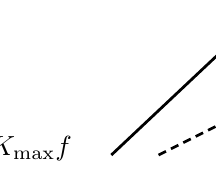
\begin{tikzpicture}\gaxesP{$K_\mathrm{max}$}{$f$}
    \draw[line width=1pt] (0.5,0) -- (2.2,1.6); \draw[line width=1pt, dash pattern=on 3pt off 2pt] (1.1,0) -- (2.5,0.7);
  \end{tikzpicture}}
  {%
  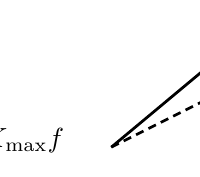
\begin{tikzpicture}\gaxesP{$K_\mathrm{max}$}{$f$}
    \draw[line width=1pt] (0.6,0) -- (2.4,1.5); \draw[line width=1pt, dash pattern=on 3pt off 2pt] (0.6,0) -- (2.4,0.9);
  \end{tikzpicture}}
  {%
  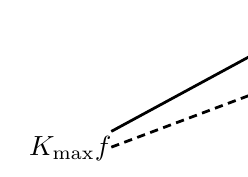
\begin{tikzpicture}\gaxesP{$K_\mathrm{max}$}{$f$}
    \draw[line width=1pt] (0,0.3) -- (2.4,1.6); \draw[line width=1pt, dash pattern=on 3pt off 2pt] (0,0.1) -- (2.4,1.0);
  \end{tikzpicture}}
  {%
  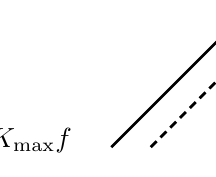
\begin{tikzpicture}\gaxesP{$K_\mathrm{max}$}{$f$}
    \draw[line width=1pt] (0.5,0) -- (2.0,1.5); \draw[line width=1pt, dash pattern=on 3pt off 2pt] (1.0,0) -- (2.5,1.5);
  \end{tikzpicture}}
\end{quizq}

% ---- Q44 (brighter light, same frequency)
\Needspace{20\baselineskip}
\begin{quizq}{}
Light shines on a metal surface and photoelectrons are emitted. The intensity of the light is increased,
but its frequency stays the same. Which row of the table is correct?
\begin{center}
  \renewcommand\arraystretch{1.7}
  \begin{tabular}{@{}p{10mm}|>{\centering\arraybackslash}p{55mm}|>{\centering\arraybackslash}p{55mm}|}
    \cline{2-3}
    & \textit{Number of electrons emitted per second} & \textit{Maximum kinetic energy of the electrons}\\ \cline{2-3}
    A. & Increases & Increases\\ \cline{2-3}
    B. & Increases & Stays the same\\ \cline{2-3}
    C. & Stays the same & Increases\\ \cline{2-3}
    D. & Stays the same & Stays the same\\ \cline{2-3}
  \end{tabular}
\end{center}
\end{quizq}

% ---- Q45 (below the threshold frequency)
\Needspace{15\baselineskip}
\begin{quizq}{}
Very bright red light shines on a metal, but no photoelectrons are emitted. Dim violet light on the same
metal does release photoelectrons. Which statement explains this?
\opts{The red light does not have enough total energy.}
  {Red light is absorbed by the metal, but violet light is reflected.}
  {Each red photon has less energy than the work function, however many photons there are.}
  {The electrons need more time to absorb the red light.}
\end{quizq}

% ---- Q46 (stopping voltage)
\Needspace{12\baselineskip}
\begin{quizq}{}
Light of frequency \qty{7.5e14}{Hz} shines on a metal with a work function of \qty{2.0}{eV}. What stopping
voltage is needed to stop all the photoelectrons?
\opts{\qty{1.1}{V}}{\qty{2.0}{V}}{\qty{3.1}{V}}{\qty{5.1}{V}}
\end{quizq}

% ---- Q47 (photon momentum)
\Needspace{12\baselineskip}
\begin{quizq}{}
What is the momentum of a photon of wavelength \qty{500}{nm}?
\opts{\qty{3.3e-40}{kg.m.s^{-1}}}{\qty{1.3e-27}{kg.m.s^{-1}}}{\qty{4.0e-19}{kg.m.s^{-1}}}{\qty{6.0e14}{kg.m.s^{-1}}}
\end{quizq}

% ---- Q48 (Einstein's explanation)
\Needspace{15\baselineskip}
\begin{quizq}{}
Which statement summarises Einstein's explanation of the photoelectric effect?
\opts{Light is a wave, and electrons absorb its energy slowly until they escape.}
  {Electrons are emitted only if the light is bright enough.}
  {Light is made of photons of energy $hf$; each photon gives all its energy to one electron.}
  {The kinetic energy of the electrons depends on the intensity of the light.}
\end{quizq}

% ---- Q49 (wave-model prediction that failed)
\Needspace{15\baselineskip}
\begin{quizq}{}
Which observation of the photoelectric effect could NOT be explained by the wave model of light?
\opts{More electrons are emitted when the light is brighter.}
  {The emitted electrons are negatively charged.}
  {Metals become warmer when light shines on them.}
  {Electrons are emitted with no measurable delay, even when the light is very dim.}
\end{quizq}

% ---- Q50 (current-voltage graphs)
\Needspace{36\baselineskip}
\begin{quizq}{}
The graph shows the photocurrent against the voltage for a photocell lit by two light beams, X and Y.
\begin{center}
  \begin{tikzpicture}
    \draw[axisline] (-2.5,0) -- (3.6,0) node[right, font=\small] {Voltage};
    \draw[axisline] (0,-0.2) -- (0,2.4) node[above, font=\small] {Current};
    \draw[line width=1pt] (-1.4,0) .. controls (-0.6,1.2) and (0,1.8) .. (1.2,2.0) -- (3.3,2.0) node[right, font=\small] {X};
    \draw[line width=1pt, dash pattern=on 3pt off 2pt] (-1.4,0) .. controls (-0.6,0.6) and (0,0.9) .. (1.2,1.0) -- (3.3,1.0) node[right, font=\small] {Y};
    \node[below, font=\small] at (-1.4,0) {$-V_0$};
  \end{tikzpicture}
\end{center}
Which row of the table correctly compares the two beams?
\begin{center}
  \renewcommand\arraystretch{1.7}
  \begin{tabular}{@{}p{10mm}|>{\centering\arraybackslash}p{50mm}|>{\centering\arraybackslash}p{50mm}|}
    \cline{2-3}
    & \textit{Frequency} & \textit{Intensity}\\ \cline{2-3}
    A. & X higher than Y & Same\\ \cline{2-3}
    B. & Same & Same\\ \cline{2-3}
    C. & X higher than Y & X greater than Y\\ \cline{2-3}
    D. & Same & X greater than Y\\ \cline{2-3}
  \end{tabular}
\end{center}
\end{quizq}

% ---- Q51 (Planck's hypothesis)
\Needspace{15\baselineskip}
\begin{quizq}{}
What did Planck assume in order to explain the black-body radiation curves?
\opts{Light travels at the same speed for all observers.}
  {Electrons orbit the nucleus in fixed paths.}
  {Light is a transverse wave.}
  {The energy of the oscillators in a black body can only take values that are whole-number multiples
   of $hf$.}
\end{quizq}

% ---- Q52 (number of photons per second)
\Needspace{12\baselineskip}
\begin{quizq}{}
A laser emits \qty{5.0}{mW} of light of wavelength \qty{650}{nm}. About how many photons does it emit
each second?
\opts{\num{3.1e-19}}{\num{1.6e13}}{\num{1.6e16}}{\num{1.6e19}}
\end{quizq}

% ---- Q53 (Kmax from the threshold wavelength)
\Needspace{12\baselineskip}
\begin{quizq}{}
A metal has a threshold wavelength of \qty{500}{nm}. Photons of energy \qty{3.5}{eV} shine on it. What is
the maximum kinetic energy of the photoelectrons?
\opts{\qty{1.0}{eV}}{\qty{2.5}{eV}}{\qty{3.5}{eV}}{\qty{6.0}{eV}}
\end{quizq}

% ---- Q54 (reading a Kmax-f graph)
\Needspace{20\baselineskip}
\begin{quizq}{}
A student plots the maximum kinetic energy $K_\mathrm{max}$ (in joules) of photoelectrons against the
frequency $f$ of the light. Which row of the table correctly identifies what the graph shows?
\begin{center}
  \renewcommand\arraystretch{1.7}
  \begin{tabular}{@{}p{10mm}|>{\centering\arraybackslash}p{45mm}|>{\centering\arraybackslash}p{60mm}|}
    \cline{2-3}
    & \textit{Gradient} & \textit{Intercept on the $f$ axis}\\ \cline{2-3}
    A. & The work function & Planck's constant\\ \cline{2-3}
    B. & Planck's constant & The work function\\ \cline{2-3}
    C. & The work function & The threshold frequency\\ \cline{2-3}
    D. & Planck's constant & The threshold frequency\\ \cline{2-3}
  \end{tabular}
\end{center}
\end{quizq}
